\documentclass[tikz]{standalone}
\usepackage{amsmath}
\usepackage{xcolor}
\usepackage{tikz}
\usetikzlibrary{arrows.meta, calc}

\begin{document}
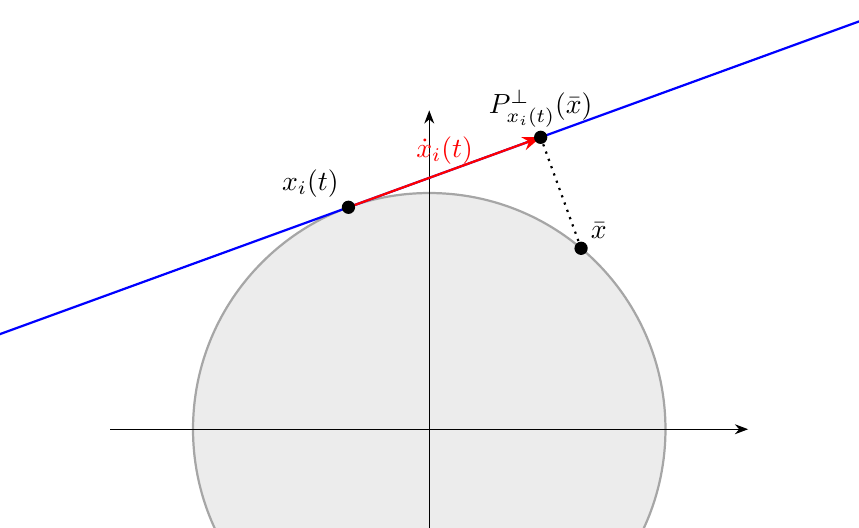
\begin{tikzpicture}[scale=3, >=Stealth]

% === Parameters ===
\pgfmathsetmacro{\anglexi}{110}
\pgfmathsetmacro{\anglemean}{50}
\pgfmathsetmacro{\tanlength}{3}  % Tangent line length
\pgfmathsetmacro{\margin}{0.7}     % Margin around figure

% === Coordinates ===
\pgfmathsetmacro{\xix}{cos(\anglexi)}
\pgfmathsetmacro{\xiy}{sin(\anglexi)}
\pgfmathsetmacro{\meanx}{cos(\anglemean)}
\pgfmathsetmacro{\meany}{sin(\anglemean)}

\coordinate (xi) at (\xix, \xiy);
\coordinate (mean) at (\meanx, \meany);

% Tangent vector at xi
\pgfmathsetmacro{\tandirx}{-sin(\anglexi)}
\pgfmathsetmacro{\tandiry}{cos(\anglexi)}

% Projection of mean onto tangent at xi
\pgfmathsetmacro{\dotprod}{\meanx*\tandirx + \meany*\tandiry}
\coordinate (proj) at ($ (xi) + (\dotprod*\tandirx, \dotprod*\tandiry) $);

% Tangent line endpoints
\coordinate (tanStart) at ($ (xi) + (-\tanlength*\tandirx, -\tanlength*\tandiry) $);
\coordinate (tanEnd) at ($ (xi) + (\tanlength*\tandirx, \tanlength*\tandiry) $);

% === Drawing region (bounding box with margin) ===
\useasboundingbox (-1-\margin,-1+\margin) rectangle (1+\margin,1+\margin);

% === Drawings ===
% Unit circle
\fill[gray!15] (0,0) circle (1);
\draw[thick, gray!70] (0,0) circle (1);

% Axes with margin
% \draw[->] (-1-\margin, 0) -- (1+\margin, 0) node[right] {$x$};
% \draw[->] (0, -1-\margin) -- (0, 1+\margin) node[above] {$y$};

% Axes with half margin
\draw[->] ({-1 - 0.5*\margin}, 0) -- ({1 + 0.5*\margin}, 0) node[right] {};
\draw[->] (0, {-1 - 0.5*\margin}) -- (0, {1 + 0.5*\margin}) node[above] {};

% Tangent line at xi
\draw[blue, thick] (tanStart) -- (tanEnd);

% Red update vector
\draw[->, red, thick] (xi) -- (proj)
node[midway, above, yshift=-1pt] {\textcolor{red}{$\dot x_i(t)$}};

% Orthogonal dotted projection
\draw[dotted, thick] (mean) -- (proj);

% Points
\fill (xi) circle (0.8pt);
\node[anchor=south east] at (xi) {$x_i(t)$};

\fill (mean) circle (0.8pt);
\node[anchor=south west] at (mean) {$\bar{x}$};

\fill (proj) circle (0.8pt);
\node[anchor=south] at (proj) {$P^\perp_{x_i(t)}(\bar{x})$};

\end{tikzpicture}
\end{document}